
\documentclass[a4paper,11pt]{article}
\usepackage{graphicx}
\usepackage{wrapfig}
\newcommand{\gtrsim}{\lower.5ex\hbox{$\; \buildrel > \over \sim \;$}}
\newcommand{\lesssim}{\lower.5ex\hbox{$\; \buildrel < \over \sim \;$}}
\newcommand\farcs{\mbox{$.\!\!^{\prime\prime}$}}% 
\pagestyle{empty}
\setlength{\topmargin}{-25mm}
\setlength{\textheight}{270mm}
\setlength{\textwidth}{180mm}
\setlength{\oddsidemargin}{-10mm}
\setlength{\evensidemargin}{-10mm}
\begin{document}

\begin {centering}
{\bf The mass distribution in quasar host galaxies revealed by quasars acting as gravitational lenses} {\bf (PI: Rusu C. E.)}\\
 \end{centering}
 
\medskip
 
{\bf Well-defined sample of gravitationally lensed quasars:} 
Since the discovery of the first gravitationally lensed quasar
Q0957+561 (Walsh et al. 1979), more than 100 strongly lensed quasars
have been discovered. They are now considered as an immensely useful astrophysical
tool, which has been providing unique insights into a broad range of
scientific problems including the fine structure of quasar accretion
disk, the structure and evolution of massive galaxies, and cosmology. 
However, a caveat is that the population of lensed quasars is quite
biased in several ways, due to the ``rare'' nature of strong lensing.
For a specific example, it has been argued that lensing galaxies should
reside in denser environments than non-lensing galaxies of similar
luminosities, because a large amount of dark matter associated with
the dense environment boosts strong lens optical depths (Oguri et
al. 2005). The fact, in turn, suggests that the mass-to-light ratios or
cosmological parameters estimated by these strong lenses can similarly
be biased. 

One can get around such lensing biases by working on a well-defined
homogeneous lens sample whose selection function is fully understood.
The current largest homogeneous lens sample is provided by the Sloan
Digital Sky Survey quasar lens search (SQLS; Oguri et al. 2006, 2008;
Inada et al. 2008), a large lens survey conduced by Dr. Oguri and his 
collaborators. We have discovered $\sim 40$ new
lensed quasars to date (e.g., Inada et al. 2009; Kayo et al. 2010),
which constitute a significant fraction of lensed quasars known. 
The selection function has been studied extensively using simulated
SDSS images (Oguri et al. 2006), allowing an accurate estimate of
lensing biases inherent to the lens sample. 

{\bf Importance of High-Resolution Images:}  
High-resolution imaging of these quasar lenses is the key to turning each
lens into a highly useful astrophysical and cosmological probe. This
is because the typical size (image separation) of a galaxy-scale strong
lenses is $\sim 1''-2''$, which is comparable to the seeing size
of ground-based imaging. The high-resolution imaging is necessary for
accurate astrometry and photometry of all lens components, two or four
quasar images accompanied by the lensed host galaxy, plus lens
galaxies in between the quasar images, all of which are confined
inside $\sim 1''-2''$ diameter. Here we highlight only two of the
many applications enabled by the high-resolution images: 

$\bullet$ Quasar host galaxies: It is very difficult to study the
properties of $z>1$ quasar host galaxies even with Hubble Space
telescope (HST) because of the cosmological surface brightness
dimming. Lensed quasars are enormously helpful to this problem,
because the lensing magnification increases both the total flux and
the apparent size of quasar host galaxies. Indeed, Peng et al. (2006)
was able to study the evolution of the black hole to bulge mass
relation out to $z\sim 4$ by using HST images of lensed quasars
(Fig.~1). The inherent idea behind such study is two-fold: First,  to infer virial masses
 for the central black holes from published spectra; second, to use lens 
 modeling in order to extract the luminosity of the 
 resolved host galaxy from under the much brighter but unresolved quasar component.

\medskip

$\bullet$ Structure and evolution of massive galaxies: Strong
gravitational lensing provides a robust mass measurement within the
Einstein radius, and hence a robust measurement of the mass-to-light
ratio for each lens. This leads to unique constraints on the
fundamental plane relation of early-type galaxies using gravitational
masses (e.g., Kochanek et al. 2000). In addition, the ensemble of strong
lenses  constrain enclosed masses at different radii, which allow us to
derive the mean radial mass profile for massive early-type galaxies
(e.g., Rusin \& Kochanek 2005). Clearly, accurate astrometric
constraints to the mass model are essential for these applications, as
well as accurate surface photometry for the lensing galaxies.

{\bf Proposed Observations:} 

- High-resolution images necessary for the applications discussed above have mainly been supplied by the HST. However, recent progress of adaptive optics (AO), especially the utilization of laser guide star (LGS), makes it possible to obtain high-resolution images using ground-based telescopes. 

- Subaru offers largest sky coverage, 11/12

- Due to the smaller diffraction limit, NIR imaging with Subaru Telescope AO has the potential to achieve {\it three times} the spatial resolution of HST.

We propose IRCS+AO188+LGS observations of 11 newly discovered candidates of foreground quasars lensing background emission line galaxies. Given the high purity demonstrated in the past, we expect that our observations will almost {\it quadruple} the number of such objects known to date.   


 galaxies
We therefore propose LGS-AO imaging of a large number (25 in total, 12 in S11A)
 of quasar lenses discovered by the SQLS,
using Subaru LGS (see Fig.~2, and also Table in the
Technical Details).

\medskip

All our targets have only ground-based images
taken with a typical seeing size of $\sim 0.9''$, and therefore imaging with LGS-AO will greatly improve relative astrometry
and surface photometry. Among 56 SQLS
lenses, 22 lenses have received high-resolution images to date. The
proposed Subaru observations will virtually double this number, significantly
increasing the sample of SQLS lenses with high-resolution imaging. 
We plan to conduct reasonably deep imaging ($\sim 20$~min or more) for each
target in order to search for lensed host galaxies down to $K \sim
21$~mag or more, a factor of $\lesssim1/10$ fainter than the quasar component
which is typical for lensed host galaxies (Peng et al. 2006). In
Figure~1 we show the source redshift distribution of some of our proposed targets,
which suggest that our targets will probe the very interesting redshift
range of $1.4 \lesssim z \lesssim 2.4$, where the scaling relation
appears to evolve quickly, as well as higher redshifts, where the uncertainty in the relation is large.  

To emphasize the critical importance of high-resolution imaging for
our study, in Figure~3 we show simulated images of a typical lensed
quasars, with and without AO. The power of high-resolution imaging is quite obvious
from this Figure; with AO, each component can be detected and studied
much more robustly and cleanly. To summarize, our proposed
observations will be an important step toward enabling full use of the
unique SQLS lens sample.  

\medskip

\begin{minipage}{\textwidth}
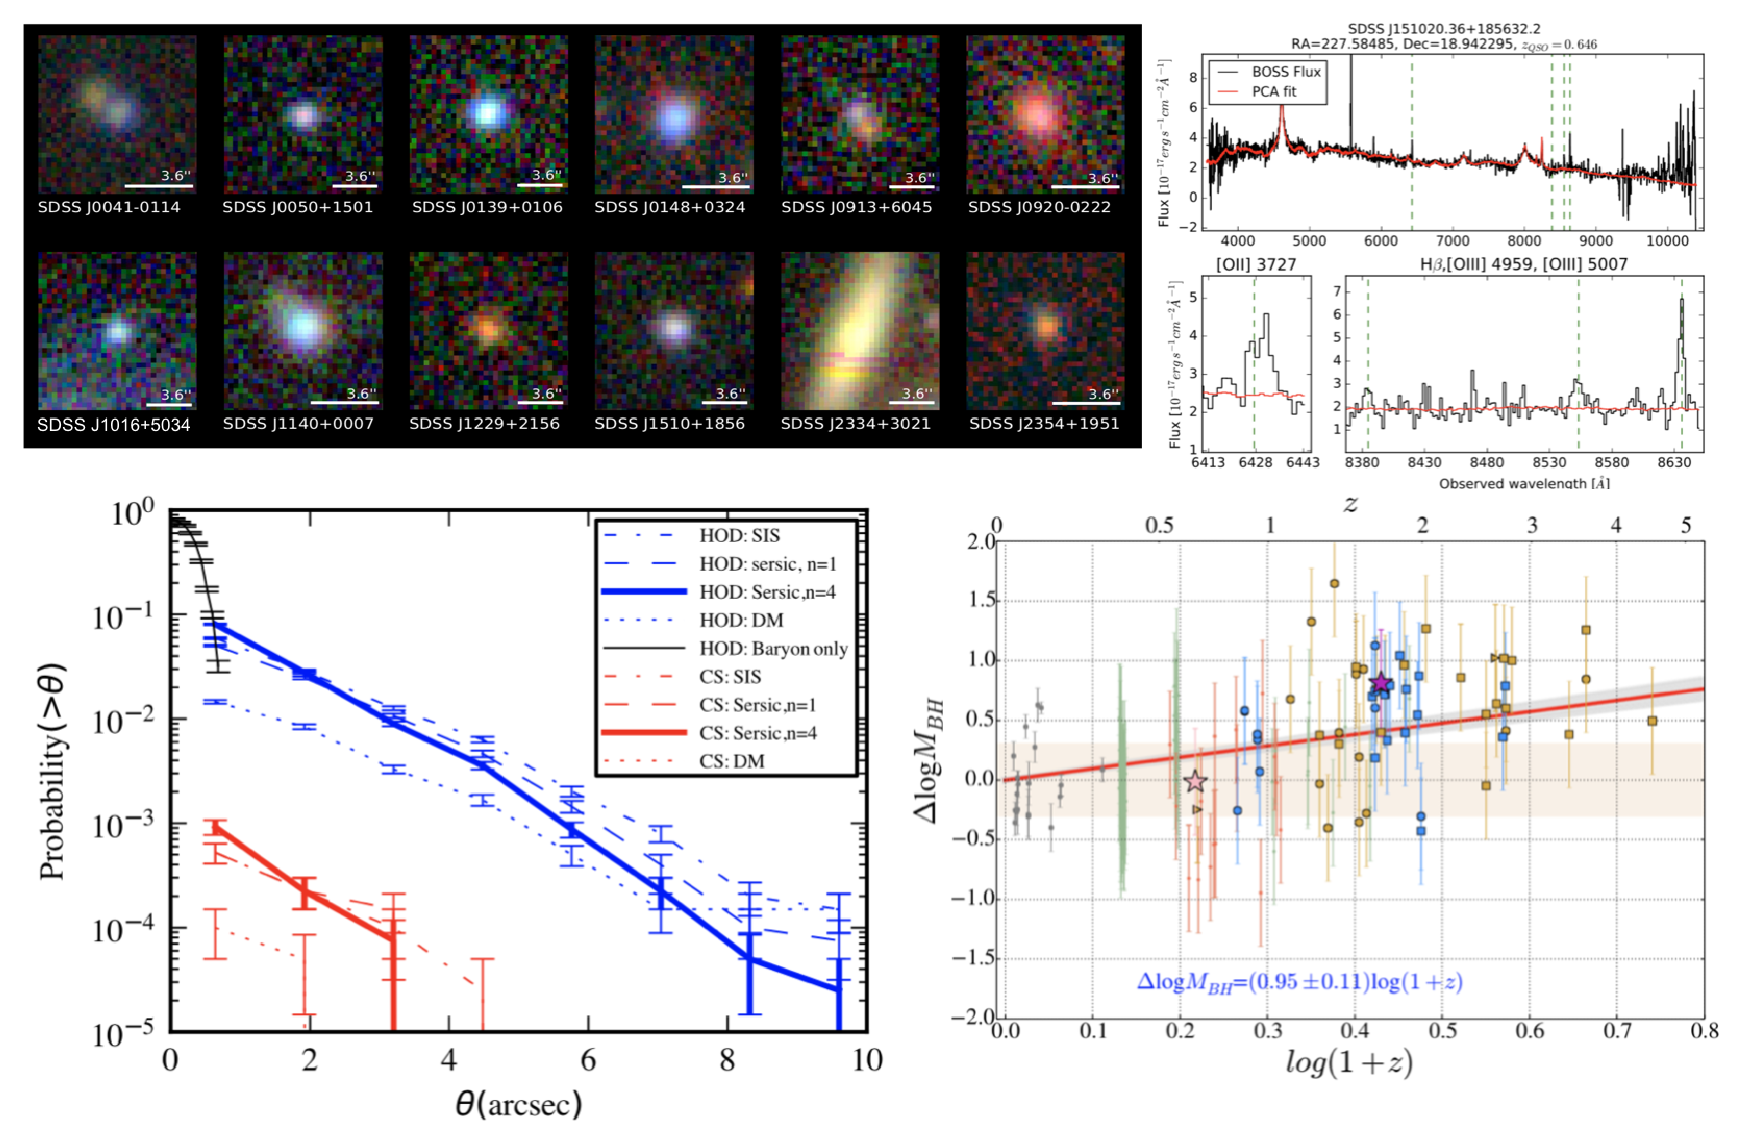
\includegraphics[width=0.95\hsize]{collage.eps}
\end{minipage}
Fig. 1: {\it Top left:} The 9+3 candidate quasars lensing emission line galaxies and LAEs, from Meyer et al. 2017. {\it Top right:} Example of the spectrum of a foreground quasar showing background emission lines, from Meyer et al. 2017. {\it Bottom left:} Probability of foreground quasars lensing galaxies, for 2 types of host dark matter halos, from Cen \& Safarzadeh 2017. {\it Bottom right:} Evolution of the offset of $M_{BH}$ in relation to the present day $M_{BH} - L_{\star}$, from Ding et al. 2017. 
  
\medskip
  
{\bf References.} Ding X., et al., 2017, MNRAS, 472, 90 $\diamond$ Cen R., Safarzadeh M., 2017, MNRAS, 467, L26 $\diamond$ Meyer R.~A., et al., 2017, arXiv:1711.01184

%{\bf References}\medskip \\ \hspace*{3mm}
%\begin{minipage}{0.48\textwidth}
%{\small
%Inada, N., et al. 2008, AJ, 135, 496\vspace{-1mm} \\
%Inada, N., et al. 2009, AJ, 137, 4118\vspace{-1mm} \\
%Kayo, I., et al. 2010, AJ, in press\vspace{-1mm} \\
%Kochanek, C. S., et al. 2000, ApJ, 543, 131\vspace{-1mm} \\
%Oguri, M., et al. 2005, MNRAS, 364, 1451\vspace{-1mm} \\
%}
%\end{minipage}
%\begin{minipage}{0.45\textwidth}
%{\small
%Oguri, M., et al. 2006, AJ, 132, 999\vspace{-1mm} \\
%Oguri, M., et al. 2008, AJ, 135, 512\vspace{-1mm} \\
%Peng, C. Y., et al. 2006, ApJ, 649, 616\vspace{-1mm} \\
%Rusin, D. \& Kochanek, C.~S. 2005, ApJ, 623, 666\vspace{-1mm} \\
%Walsh, D., et al. 1979, Nature, 279, 381\vspace{-1mm} \\
%}
%\end{minipage}

\end{document}
